\documentclass[11pt]{article}
\usepackage[T1]{fontenc}
\usepackage{times}%, babel}
\usepackage{secdot,natbib}
\usepackage{latexsym, amsthm, amsmath, amssymb, color, rotating, multirow, graphicx, hhline, array, tablefootnote}
\usepackage{scalefnt, enumerate}
\usepackage{footnote}
\usepackage{threeparttable,booktabs}
\usepackage{natbib}
\usepackage[hyphens]{url}
%\usepackage{bm, url}
%\usepackage{slashbox}
\usepackage{tikz,pgfplots}
%\usepackage{subcaption}
\usepackage[margin=10pt,font=small,labelfont=bf,labelsep=endash]{caption}
\usepackage{subfigure}

\usepackage{kotex} %Korean TeX
%\usepackage[latin9]{inputenc} % kotex package와 충돌. 향후 kotex 삭제하면 될 듯.




%%% ----------------------------------------------------------------------
%\clubpenalty=10000 \widowpenalty=10000
%\renewcommand{\baselinestretch}{1.5}
% \renewcommand{\theequation}{{\rm \thesection.\arabic{equation}}}
\renewcommand{\theequation}{{\rm \arabic{equation}}}
\oddsidemargin 0in  %.10in
\evensidemargin 0in
\hyphenpenalty 2000

\textwidth 6.5in    %6.5
\textheight 8.75in     %8.5
\topmargin 0.0in      %0in
\headsep 0in \makeatletter
\newcommand{\singlespacing}{\let\CS=\@currsize\renewcommand{\baselinestretch}{1.1}\tiny\CS}
\newcommand{\doublespacing}{\let\CS=\@currsize\renewcommand{\baselinestretch}{1.5}\tiny\CS}
\newcommand{\realdoublespacing}{\let\CS=\@currsize\renewcommand{\baselinestretch}{2.0}\tiny\CS}
\newcommand{\mydoublespacing}{\let\CS=\@currsize\renewcommand{\baselinestretch}{1.499}\tiny\CS}

\newtheorem{theorem}{Theorem}[section]
\newtheorem{proposition}[theorem]{Proposition}
\newtheorem{lemma}[theorem]{Lemma}
\newtheorem{corollary}[theorem]{Corollary}

\def\N{\mathbb{N}}
\def\1{\mathbf{1}}
\def\P{\mathbf{P}}
\def\E{\mathbf{E}}
\newcommand{\maximize}{\mathop{\mbox{{\rm maximize}}}\limits}
\newcommand{\minimize}{\mathop{\mbox{{\rm minimize}}}\limits}
\newcommand{\argmax}{\mathop{\mbox{{\rm arg\,max}}}\limits}


%\newcommand\ks[1]{{\textbf{#1}}}
\newcommand{\ks}[1]{{\color{blue} #1}}
\newcommand{\ju}[1]{{\color{magenta} #1}}
\newcommand{\yj}[1]{{\color{red} #1}}


\setlength\parindent{0cm}
\setlength{\parskip}{12pt}%

\renewcommand\ttdefault{cmvtt}

%%%%%%%%%%%%%%%%%%%%%%%%%%%%%%%%%%%%%%%%%%%%%%%%%%%%%%%%%%%%
\begin{document}

\begin{center}
{{\Large \bf Response to Review Reports on POM-Jul-20-SI-0934.R3}\\[6mm]
{\LARGE ``Sharing Economy in the Cloud:\\ Pricing Schemes for Peer-to-Peer Storage Platforms''}\\[15mm]}
\end{center}

\baselineskip 18pt

\noindent \underline{\large \bf General Response to the Review Team}

\ju{(DE한테 SE 기 살려주기)}

\newpage





%%%%%%%%%%%%%%%%%%%%%%%%%%%%%%%%%%%

\noindent \underline{\large \bf Authors' Response to SENIOR EDITOR}\\[-11mm]

%%%%%%%%%%%%%%%%%%%%%%%%%%%%%%%%%%%
\begin{quotation}
{\em
\noindent \textbf{Senior Editor: } This is an R3 paper. On one hand, the authors' efforts are well-appreciated. On the other hand, the paper seems to be still not yet publishable. It is disappointing.
It happens that one critical reviewer who voted for rejection last time is not available. As a result, a new reviewer is invited to help. The comments are not positive. While I feel it is fair for the authors to have one last chance to improve the work faithfully. If they choose to do so, please work really hard to improve the paper as much as possible for the highest standard. Next round, we will make a decision on either accept or reject.
}
\end{quotation} \vspace{-4mm}

\ju{지금까지 긴 review round를 올바른 방향으로 잘 이끌어줘서 너무 감사하다. 그리고 가장 생산적인 comment를 제공해왔던 R2에게서 accept 결정을 받은 것에 대해서도 고무적으로 생각한다.}

\ju{다만 4라운드까지 가는 과정에서 완벽한 퀄리티를 만들어내지 못한 점에 대해서는 미안하게 생각한다. 새로운 R3가 생산적인 코멘트를 많이 제공해주었고, 또한 우리의 기존 writing에서 중대한 오해를 발생시키는 부분이 있다는 것을 알게되었다.}

\ju{Most importantly, 우리가 'hybrid' pricing에 대해 명확하게 표현하지 않은 점 때문에 오해가 발생했던 것 같다. Hybrid pricing은 여러 옵션을 동시에 주는 것이 아니라 그 구조가 subscription과 two-part tariff의 성격을 동시에 갖는 것인데, 이것이 제대로 전달되지 않은 것 같다. 긴 라운드 동안에 너무 response letter를 통해서 review team에게 잘 전달하려는 데에만 집중해, 정작 manuscript에서 이러한 부분이 깔끔하게 설명되지 못한 점 정말 죄송하다. 이것은 SE 및 referee의 올바른 가이드에도 불구하고, 새로운 reader들을 충분히 고려하지 못한 우리의 불찰이다.}

\ju{물론 R3는 전체적으로 논문에 대한 매우 좋은 이해도를 바탕으로, 생산적인 코멘트를 주었다. 특히 R3가 직접 제시한 논문들 역시 (좀 다르지만) 연관이 있었고, technical한 부분에서 아주 중요한 부분들을 짚어주었다. 우리 결과에서 unrealistic한 케이스들이 배제된다는 것을 더 강조했어야 했는데(...)}

%%%%%%%%%%%%%%%%%%%%%%%%%%%%%%%%%%%%%%%%%%%%%%%%%%%%%%%%%

\begin{quotation}
{\em
\noindent \textbf{Senior Editor (Point 1): }
In addition to addressing the review comments, please pay attention to the following:
We need a complete picture of the study. What are the key insights? What is the core conclusion. They should be clearly presented in a coherent way. We need a beautiful picture and a perfect paper.
}
\end{quotation} \vspace{-4mm}

\ju{(나중에 생각해보자)}
2023.01.09
i) 단순히 pricing이 아니라 어떠한 pricing scheme을 가져가는지를 결정하는 것이 중요하다.\\
ii) pricing scheme을 설정하는 과정에서, two-sided platform의 경우에는 양쪽의 incentive를 모두 고려해야하기에 단순히 renter의 입장에서의 surplus를 확보하는 subscription 등의 pricing scheme보다는, 오히려 provider에게 충분한 보상을 주는 형태의 pricing scheme을 책정하는 것이 훨씬 total surplus 차원에서 유익할 수 있다.\\ 
(특히, provider와 renter가 단순 1:1 매칭이 되는 것이 아닌 조금 더 복잡한 경우...? or renter의 사용량에 따라서 provider에게 비용이 부과 되는 경우...? - 여하튼 이러한 경우에는 이 결정이 더 복잡할 수 있다? )

%%%%%%%%%%%%%%%%%%%%%%%%%%%%%%%%%%%%%%%%%%%%%%%%%%%%%%%%%
\textbf{Implications to practices:}
\begin{quotation}
{\em
\noindent \textbf{Senior Editor (Point 2): }
 What is the big deal of the findings? What real world practices can be improved with respect to the theoretical findings? Some real-name companies' practices should be explained/challenged by using the derived findings in the paper. This demonstrates the applications of the findings from this piece of research.
}
\end{quotation} \vspace{-4mm}

\ju{가격 체계를 어떤 걸 결정하느냐 자체가 중요하고, 이게 supply 단에 따라 달라질 수 있다}
2023.01.23\\
실제 회사 케이스를 어떻게 가져갈까요? - renter의 사용량에 따라 비용이 부과되는 형태면 좋을 것 같은데... uber? - uber 기존 논문들이 거리 상관 없이 fixed price였던 것 같은데, 이 부분 관련에서 언급할만한 부분이 있을까요?


%%%%%%%%%%%%%%%%%%%%%%%%%%%%%%%%%%%%%%%%%%%%%%%%%%%%%%%%%
\textbf{Contribution to literature: }
\begin{quotation}
{\em
\noindent \textbf{Senior Editor (Point 3): }
More discussions on how the findings supplement or challenge the prior studies in the OM literature should be explained. As the new reviewer points out, many important works are missing in the literature review and the current paper's novelty is under doubt. This will better highlight the paper's positioning in the OM literature.
}
\end{quotation} \vspace{-4mm}

\ju{지난 리뷰에서도 최신 논문들을 추가하면서 계속 follow-up을 했었다. 이번에 제시된 indirectly related paper를 추가하는 것이 매우 도움이 되었으나, 그것이 전체적인 literature stream을 바꾸지는 않았다. Segmentation 관련된 것은 miscommunication issue}

2023.01.03\\
4th-response 추가 내용\\
``Prior studies on pricing in the sharing economy, such as Cachon et al. (2017) and Zhang et al. (2022), did not consider the potential of the pricing schemes that we have examined in this paper. Specifically, these studies postulated a common price and focused on price-wage relationships---i.e., how the platform should share its revenue with workers---rather than on how to price services depending on usage levels. Consequently, these studies paid scant attention to comparing service pricing schemes, such as a two-part tariff, subscription-based pricing, and hybrid pricing.'' (page 7)


추가 literature :
Guda, Harish, and Upender Subramanian. "Your uber is arriving: Managing on-demand workers through surge pricing, forecast communication, and worker incentives." Management Science 65.5 (2019): 1995-2014.\\
위 내용은 A / b 존이 나눠져있는 상황에서.... 다루는 문제 같은데, 저희 논문의 컨셉 자체를 ONLINE으로 가져가면서
i) 거리 문제가 전혀 없음 ii) provider:renter이 다:1 매칭 필요, iii) renter의 사용량에 따른 비용 부과, iv) 시스템 안정성을 위한 structure 설계 필요...?(theta, t...) 등을 가져갈 수 있으려나요?\\
현재 전반적으로 resource를 sharing하는 것에 대해서 트렌드(?)처럼 가고 있는 것 같은데, cloud storage가 아닌 colud computing 등을 예시로 들면서, 이 시장이 더 커질 수 있다는 식으로 갈 수 있을까요?

읽어보면 좋을듯요!
https://www.techradar.com/reviews/storj-decentralized-cloud-storage\\
https://blocksandfiles.com/2022/11/08/storej-gives-the-lowdown-on-web-3-0-decentralized-storage/
%%%%%%%%%%%%%%%%%%%%%%%%%%%%%%%%%%%%%%%%%%%%%%%%%%%%%%%%%
\textbf{Model: }
\begin{quotation}
{\em
\noindent \textbf{Senior Editor (Point 4): }
Please explain the physical meaning of different model settings clearly. This is in line with the reviewer's comments on the "invest in no redundancy" case.
}
\end{quotation} \vspace{-4mm}
$\theta = 0$ 자체는 말이 안되는 케이스. invest in no redundancy는 nonsense. 현재 $\theta - t$의 경우에는 현업에서 '000'와 같은 형태로 가져가고 있으며, $\theta$는 유지하면서 $t$를 낮출 수 있는 방향(혹은 안정성에 대한 기준 threshold를 더 높일 수 있는 방향)에 대한 지속적인 고민을 하고 있음. \\
현재 일정 시스템을 안착한 후, $\theta - t$에 대해서 어느정도 유지하고 있기는 한데, 이는 현재 시스템으로 충분한 안정성이 확보되었기 떄문이라고 생각.
\newpage
%%%%%%%%%%%%%%%%%%%%%%%%%%%%%%%%%%%%%%%%%%%%%%%%%%%%%%%%%%%%%%%
\noindent \underline{\large \bf Authors' Response to Reviewer 2}
%%%%%%%%%%%%%%%%%%%%%%%%%%%%%%%%%%%%%%%%%%%%%%%%%%%%%%%%%%%%%%%


%%%%%%%%%%%%%%%%%%%%%%%%%%%%%%%%%%%%
\begin{quotation}
{\em
\noindent \textbf{Reviewer 2: }
Accept.}
\end{quotation}\vspace{-4mm}

\ju{Thank you (...)}

\newpage
%%%%%%%%%%%%%%%%%%%%%%%%%%%%%%%%%%%%%%%%%%%%%%%%%%%%%%%%%%%%%%%
\noindent \underline{\large \bf Authors' Response to Reviewer 3}
%%%%%%%%%%%%%%%%%%%%%%%%%%%%%%%%%%%%%%%%%%%%%%%%%%%%%%%%%%%%%%%

\begin{quotation}
{\em
\noindent \textbf{Reviewer 3: }
This paper studies different pricing strategies a firm facing heterogeneous consumers might consider. In particular, consumers vary in the extent they will use the firm’s service, and the firm charges consumers either (i) a pure subscription fee, (ii) a subscription fee and a usage fee, or (iii) a subscription fee, a usage fee, and a quantity of free usage.
The authors study these different pricing schemes in the context of a firm that relies on independent
providers to provide the capacity required to serve consumers. In the main analysis, the different
pricing schemes may affect providers because they are paid according to a fixed commission. The paper’s particular focus on peer-to-peer file storage platforms adds an additional firm lever – the extent to which files are redundantly stored.
The paper compares the pricing schemes by profitability and surplus generated under two conditions – one in which providers are plentiful and one in which they are not. When providers are plentiful, the two part tariff is the most profitable while the subscription model is the least (ordering is reversed for
surplus). When providers are not plentiful, the paper provides a partial ordering.

This is the third round of review for this paper, and it appears that the review team has reached a
certain degree of convergence. This is the first round that I am participating in the review of this paper, so I leave it to the editors to determine which of my comments are appropriate for the authors to address at this stage in the process. Unfortunately, in my opinion this paper is not yet ready for publication.
}
\end{quotation}\vspace{-4mm}

\textbf{Literature Review:}
\begin{quotation}
{\em
\noindent \textbf{Reviewer 3  (Point 1): }
This is fundamentally a paper about market segmentation. Yet the paper is not at all grounded in this vast literature. What would this literature predict about the relative profitability of the
pricing schemes considered here? Why does the sharing economy/online platforms/peer-to-peer file
sharing context change those predictions? Without answering these questions, it is impossible for the reader to assess the contribution of this paper.
In addition to this classic literature, there is a broad literature at the intersection of operations and marketing that studies subscriptions (e.g., Cachon \& Feldman, 2011). Similarly, there are papers that
study subscription pricing with limits on usage (e.g., Randhawa \& Kumar, 2008). It is the authors’
responsibility to thoroughly review these literatures.
}
\end{quotation}\vspace{-4mm}

\ju{다음 response와 관련해서...segmentation은 아님}

\ju{Two-sided에서는 supply의 부족 때문에 가격을 맞춰줘야 하는 부분에서 welfare의 order가 달라질 수 있다.}

일반적인 market에서는 pricing scheme을 고려할 때, 오직 profit에만 초점을 맞추지 굳이 surplus를 고려하지는 않음 - surplus를 고려한 literature가 어떤 것 있는지는 확인 필요 -. 하지만, 우리는 two-sided platform이기에 토탈 surplus를 고려할 필요가 있음\\
Huh, Woonghee T., and Hongmin Li. "Product‐line pricing with dual objective of profit and consumer surplus." Production and Operations Management.
위 논문 저 access가 안되는데 한번 확인 부탁드려요 ㅠㅠ

%%%%%%%%%%%%%%%%%%%%%%%%%%%%%%%%%%%%%%%%%%%%%%%%%%%%%%%%%%%%%%%
\textbf{Results:}
\begin{quotation}
{\em
\noindent \textbf{Reviewer 3  (Point 3): }
1. Why is the hybrid pricing scheme (a subscription fee, a usage fee, and a quantity of free usage) not the most profitable pricing scheme? My intuition is that the most profitable scheme would impose a different total cost to each type
of consumer (where types are based on their
exogenous usage type). The hybrid pricing scheme offers the greatest ability to do this (it segments the market into three groups instead of two (with two part pricing) or one (with subscription pricing). Is this the result of requiring the initial consumption to be free? What if the firm solved the more general problem of determining (i) the subscription price), (ii) the usage fee for the first $x$ units of usage, and (iii) the usage fee for the remaining units of usage? 
}
\end{quotation}\vspace{-4mm}
\ju{다시 꼼꼼히 읽어봅시다. Hybrid 자체는 제대로 이해한 것 같기도 한데? 우리 세팅에서 two-part tariff >= hybrid가 되는 것에 대해 R3가 얘기한대로 free amount를 결정할 수 있으면 hybrid > two-part tariff가 아니냐고 질문을 가질 수 있을 것 같음. 물론 우리 결과 상으로는 그런 상황에서도 hybrid가 two-part를 뛰어넘을 수 없다는 걸 보일 수 있으니 잘 설명해주면 될 것 같음.}

우리가 제시하는 hybrid pricing scheme는 서로 다른 개인에게 다른 형태의 pricing을 제공하는, 두 pricing을 맞춤형으로 제공하는(self selection이 발생하는)형태를 의미하는 것이 아님. subscription과 two-part tariff 사이에서, 일부만 무료로 제공한다는 '특정, 정해진' pricing scheme. 따라서 당연히 most profitable한 것을 보장하지는 않음. 이러한 pricing을고려한 이유는 intuitive한 관점에서 subscription은 renter, two-part tariff는 prvider 에게 가장 매력적인 요금 체계로 보일 수 있어 그 사이의 가격 구조를 고려한다는 점, 그리고 실제로 이렇게 partially하게 무료로 제공하는 요금제들이 많다는 점이 있음. hybrid pricing scheme이라는 용어로 인하여 혼동을 준 것은 정말 미안함.

\ju{Hybrid 기존 논문에 있었는지 체크, 있었으면 quote 가져오기 // Cap + pay-per-use}

위 내용에서 강조가 되어야할 부분이 'some hybrid pricing scheme'이라는 부분인 것 같아요. 이 hybrid에서 얼마나 무료로 줄 것인지를 select하는 모델로 생각해버리면서 나오는 misunderstand일 가능성도..?

%%%%%%%%%%%%%%%%%%%%%%%%%%%%%%%%%%%%%%%%%%%%%%%%%%%%%%%%%%%%%%%
\begin{quotation}
{\em
\noindent \textbf{Reviewer 3  (Point 4): } 2. Theorem 1 indicates that the firm invests in no redundancy, i.e. $\theta = 0, t = 0$. What does this mean in practical terms? That the firm deletes the files that consumers try to store on it? That consumers can never retrieve their files? Or are there unstated constraints (e.g., $\theta$ > 1) that avoid some of these nonsense outcomes? It is worth noting that Theorem 1 follows from the fact that consumers do not care directly about redundancy. In practical terms, this means they don’t care if their file gets deleted; in mathematical terms this means that $\theta$ appears in their
utility only when scaled by another decision variable, the subscription price. Note that this is also true of providers – is the firm’s objective changed at all by varying the level of $\theta$?
}
\end{quotation}\vspace{-4mm}
$\theta = \frac{m}{k}$ where $m > k$는 명시 되어 있음. 다만, $\theta >1$이 명시되어있지는 않음. 이 부분에서는 더 자세히 써줘야 했는데 죄송하다는 식으로의 서술이 필요하지 않을까 싶음.\\
마찬가지로 uptime $t$가 0보다 크다는 것이 명시적으로 써져있지는 않음. 이 부분은 더 명시적으로 써져있지 않기에 $\theta \psi(t)$를 minimize 하는게 t=0일 수 있찌 않느냐($\psi(0) = 0$이라는 가정 하에)는 말이 logically make sense 하기는 함.\\
이 부분에 대해서는 i) $\theta > 1$, $t>0$은 명시적으로 다시 한 번 언급 ii) $\theta$와 $t$가 만족하는 관계를 조금 더 강조하면서, $t$가 지나치게 작아지는 것은 너무나도 큰 $\theta$의 증가를 요구하는 과정이 됨. 
을 강조할 필요가 있어 보임

질문으로 나와있는 의미에 대한 답변은 차례대로는,\\ i) $\theta = 0, t=0$등은 말이 아예 안되는 조건, 당연히 practical term도 존재하지 않음 \\
ii) consumer 는 redundancy에 따라서 비용이 증가되는 부분이 있으므로 실제로 고려 대상임.\\
iii) file delete는 매우 민감한 사항이므로, platform이 이러한 경우를 아예 발생 안하도록 세팅(이 부분은 우리가 가정한 $\theta t$ 관계와도 연결) \\
iv) provider는 $\theta$가 증가함에 따라서 저장에 대한 수익 증가 / 다운로드에 대한 수익 감소(할당 확률 감소) / 비용 감소 등의 직접적인 연결이 발생\\
v) platform 입장에서는 안정적인 운영일 위한 structure를 구성해야 할 필요가 있고, 이와 동시에 player들인 renter과 povide에게 부담을 주는 코스트를화최소화 해야 할. 의무가 있음. 하지만, 이 둘 사이의 cost는 tradeoff가 있으므로 신중한선택 필요

%%%%%%%%%%%%%%%%%%%%%%%%%%%%%%%%%%%%%%%%%%%%%%%%%%%%%%%%%%%%%%%


\begin{quotation}
{\em
\noindent \textbf{Reviewer 3  (Point 5): }
3. The results presented are incomplete – in the “market clearing” case, the authors do not
provide a complete ordering of the profitability (or surplus generation) associated with each
pricing option. How can a firm use this research to choose a pricing strategy without a complete
ordering?
}
\end{quotation}\vspace{-4mm}

\ju{Stereotype과 달라지는 결과를 보여준 것이 중요하다 ... 그것이 우리 핵심 메시지다}

\ju{Ordering이 clear하지 않는 구간이 있음 -> numerical 예시도 간단히 보여줄수도}

이 부분은 se한테 쓴 내용 참조

%%%%%%%%%%%%%%%%%%%%%%%%%%%%%%%%%%%%%%%%%%%%%%%%%%%%%%%%%%%%%%%

\textbf{Model:}
\begin{quotation}
{\em
\noindent \textbf{Reviewer 3 (Point 6): }
1. Why are individual providers assigned the same amount of files to store? Shouldn’t providers offer different amounts of storage capacity according to their individual storage costs?
}
\end{quotation}\vspace{-4mm}

response 3rd에 있는 질문 발췌(예시)\\
이 내용 바탕으로 답변 달면 되지 않을까요?\\
Both reviewers continue to have concerns with the model setup. 
(a) Heterogeneity of users: As R2 points out, users (both renters and providers) can be heterogeneous in other dimensions as well, which is a good observation. The authors are encouraged to explore possible models which consider heterogeneity in multiple dimensions. However, I would think that the review team will also be fine if the authors can only incorporate some heterogeneity into the model (e.g., the heterogeneity the current model considers). If they take this approach, the authors should elaborate on at least the following two aspects---why the authors consider this specific heterogeneity against other possible heterogeneity, and how the chosen model setup (i.e., ignoring the other possible heterogeneity) affects the main insights.  

만약, 'individual storage cost'가 각 provider들이용량을 제공하는 '비용'이 다르다는 것을 의미하는 것이라면... 이건 어차피 idle space를 제공하는 것이라서 크게 차이가 없다는 식으로 답변하면 되지 않을까 싶습니다.

\ju{round 3에서 three dimensions에 대한 heterogeneity 반영 때문에 ...}


\textbf{2023.01.15 추가.}\\
response 3rd general response:\\
\textbf{\large 2. Examining the Validity of the Findings}

\textbf{2.1. Additional Heterogeneity Dimensions}\\
Related to: \textbf{[SE Point 2a] [R2 Point A2a] [R2 Point A2b] [R2 Point A4a] [R2 Point A4b]}

The review team suggested additional possibilities of the renter/provider heterogeneity, which provided valuable directions to further convince our results. However, it is worth noting that our main model already accounts for three important sources of heterogeneity—two dimensions of renter heterogeneity (download frequency, utility per download) and one dimension of provider heterogeneity (operating costs). Therefore, we have maintained and justified the current model's peer heterogeneity and discussed the potential consequences of additional  possibilities.

To further validate our findings, we have also conducted several numerical analyses. Specifically, we have examined various scenarios on renters' storage volume, bandwidth volume, and utility per unit bandwidth volume. The results show that our findings remain consistent across all heterogeneity sources and scenarios we have considered.



\begin{quotation}
{\em
\noindent \textbf{Senior Editor (Point 2a): } Both reviewers continue to have concerns with the model setup. 
(a) Heterogeneity of users: As R2 points out, users (both renters and providers) can be heterogeneous in other dimensions as well, which is a good observation. The authors are encouraged to explore possible models which consider heterogeneity in multiple dimensions. However, I would think that the review team will also be fine if the authors can only incorporate some heterogeneity into the model (e.g., the heterogeneity the current model considers). If they take this approach, the authors should elaborate on at least the following two aspects---why the authors consider this specific heterogeneity against other possible heterogeneity, and how the chosen model setup (i.e., ignoring the other possible heterogeneity) affects the main insights.  }
\end{quotation} \vspace{-4mm}

We sincerely appreciate the review team's constructive comments on various dimensions of heterogeneity. Considering that our main model already accounts for three important sources of heterogeneity---two dimensions of renter heterogeneity (download frequency, utility per download) and one dimension of provider heterogeneity (operating costs), we have decided to adopt the second approach, which maintains and justifies the current model's user heterogeneity and investigates with the discussion on the consequences of other heterogeneity. In addition, we have shown that our findings remain consistent even when such additional heterogeneity is considered by conducting numerical analyses. Below, we have summarized how we have addressed each point in this revision.

\textbf{Heterogeneity of Renter's Storage Volume.} Reviewer 2's \textbf{Point A2a} suggested that renters' storage volumes are substantially heterogeneous, leading to various renter segments---e.g., renters with large storage volume and low frequency download request, and those with small storage volume and highly frequent download request. We admit that ignoring this heterogeneity is a big missing point, and thus, we need to understand its potential consequences. We have addressed this point by conducting a numerical analysis that incorporates such renter segments. The results suggest that the main insights from the basic setup remain unchanged under several conditions where various segments coexist in the market. Please refer to our responses to Reviewer 2's \textbf{Point A2a} for the technical details.

\textbf{Heterogeneity of Renters' Bandwidth Volume.} Our model already accounted for the heterogeneous download frequency and utility per volume. In this revision, we have numerically tested whether our findings remain consistent when we consider an additional dimension or an alternative functional form of heterogeneity. As noted by Reviewer 2's \textbf{Point A4a}, the independence assumption between a renter's bandwidth utility and her download frequency may not hold in practice. We have numerically analyzed the consequences of assuming a positive correlation between utility per download and download frequency and obtained consistent results. Also, Reviewer 2's \textbf{Point A4b} pointed out that the current parametric assumption may drive our findings. Hence, we have conducted a numerical study on whether other functional forms of download frequency yield the same or different insights. By testing other parameter values of the Pareto distribution ($b$), which manipulate the proportion of high-frequency renters, we have obtained qualitatively consistent results across all tested scenarios. 

\textbf{Heterogeneity of Provider's Storage Volume.} Reviewer 2's \textbf{Point A2b} indicated that the assumption that each provider supplies a unit volume of unused capacity requires a condition: the provider's income and cost are both proportional to the volume of the capacity provided. Accordingly, we have provided this assumption's specific justification and potential consequences when this assumption does not hold. To summarize, our assumption is plausible for the following reasons. First, several sources of operating costs are proportional to bandwidth usage, e.g., bandwidth and electricity costs. Second, bandwidth usage is likely proportional to storage volume because P2P storage platforms tend to assign more contracts to high-volume providers. Please refer to our responses to Reviewer 2's \textbf{Point A2b} and the revised manuscript for more details. 



\begin{quotation}
{\em
\noindent \textbf {Reviewer 2 (Point A2a): }2. The assumptions that a renter needs a storage space for her unit volume of files and that the provider can share his unit volume of storage space need a second thought. 

a. As can be seen, the model focuses on the heterogeneity of renters’ bandwidth usage level only, while the heterogeneity of their storage volume is absent due to the assumption of unit volume per renter. This assumption takes away an important tradeoff from the model. In reality, there are renters with large storage volume and low frequency of download request versus renters with small storage volume and  high frequency download request. The specific pricing scheme must have different impacts on renters with different storage and bandwidth needs, thus affecting the segmentation of renters. In short, I wonder whether the authors could build their model based on heterogeneity of not only bandwidth usage but also storage volume.
}
\end{quotation}\vspace{-4mm}
 
We take your point, and we agree in retrospect that the implications of pricing schemes might be different across renter segments depending on their storage and bandwidth needs. Although we could not reflect this heterogeneity in our main model in addition to the three existing dimensions---renters' utility per bandwidth volume, bandwidth request frequency, and providers' operating costs, we have numerically examined the cases where different segments of renters in terms of storage volume and download requests coexist in the market. Our findings obtained from numerical analyses suggest that the main insights from the basic setup remain unchanged. Below, we have summarized their conditions and results.

%Let us summarize key findings from our additional analyses. We have found that the main insights from the basic setup remain unchanged. Interestingly, depending on how the platform designs hybrid pricing, the influence of hybrid pricing can become similar to that of a two-part tariff because a larger portion of renters demands more bandwidth volume than the bandwidth allowance. We have obtained these findings based on numerical analyses and summarized their conditions and results below.

\textbf{Generalized utility function.} % (우리가 main model에서는 unit volume인 renter들의 utility function만을 다루었기에) renter의 heterogeneity를 반영하기 위해서는 먼저 unit volume이 아닌 renter들의 utility function의 define 이 필요하다. 이를 define하기 위해서 용량이 v_i이고 frequency가 \lambda_i인 renter를 가정해보자. 우리는 이들의 utility function을 define하는 관점에서 1) net utility가 volume에 비례한다고 가정을 하였다. 2) 저장 비용은 당연히 volume에 비례한다. 3) bandwidth volume은 frequency가 \lambda_i이고 용량이 1인 renter의 v_i배가 된다.
Since the utility functions in our main model concern renters with a unit storage volume only, we need to define new utility functions for renters with heterogeneous storage volume. To do this, we have considered renter $i$ having storage volume $v_i$ and frequency $\lambda_i$. For this renter's utility function, we have assumed that 1) the benefit from P2P storage is proportional to $\lambda_i v_i$, 2) the storage cost is proportional to $v_i$, and 3) the bandwidth volume is $v_i$ times of the unit-volume renter with $\lambda_i$.

% 따라서 bandwidth fee가 없는 subscription이나 비례해서 부과하는 two-part tariff의 경우에는 전체 utility function 자체가 용량이 1인 경우의 v_i배가 된다고 할 수 있다. 하지만 hybrid pricing의 경우에서는 무료 용량이 어떻게 제공되는지에 따라서 utility function도 달라질 수 있다.
Based on these assumptions, we have seen that for the two-part tariff and subscription-based pricing, the new utility function is $v_i$ times of the previous function for a unit storage volume. However, the hybrid pricing might have various utility forms regarding how to price bandwidth services. For instance, the platform may offer the volume of bandwidth allowance proportionally to storage volume, which is widely observed in cloud service contracts. Also, the platform may provide the volume constantly across all renters regardless of their storage volume.

Since these possibilities seem plausible, we have examined both cases to explore the implications of hybrid pricing in the new setting. Below, we have specified the renter's utility functions in the current model and the extended ones that account for volume heterogeneity.

Here are the current utility functions of renters by pricing scheme:
\begin{equation*}
    U_i = \begin{cases}
    \lambda_i u_i - \theta p_s &\text{ under the subscription-based pricing,}\\
    \lambda_i u_i - \theta p_s - \max\{\lambda_i - q \lambda_0, 0\}p_b &\text{ under the hybrid pricing,}\\
    \lambda_i u_i - \theta p_s - \lambda_i p_b &\text{ under the two-part tariff.}
    \end{cases}
\end{equation*}
Henceforth, we generalize those functions for renter $i$'s storage volume $v_i$. First, when the bandwidth allowance is proportional to $v_i$, we can rewrite the functions as follows (\textbf{Utility Function I}):
\begin{equation*}
    U_i = \begin{cases}
    \lambda_i u_i v_i- \theta v_i p_s &\text{ under the subscription-based pricing,}\\
    \lambda_i u_i v_i- \theta v_i p_s - \max\{\lambda_i v_i - q \lambda_0 v_i, 0\}p_b &\text{ under the hybrid pricing,}\\
    \lambda_i u_i v_i- \theta v_i p_s - \lambda_i v_i p_b &\text{ under the two-part tariff.}
    \end{cases}
\end{equation*}
If $\lambda_0$ is independent of $v_i$, the utility is proportional to $v_i$ for all pricing schemes. Therefore, mere differences in storage demand do not affect a renter's adoption decision in this situation.

Second, we can rewrite the utility functions when the bandwidth allowance is constant as follows (\textbf{Utility Function II}): 
\begin{equation*}
    U_i = \begin{cases}
    \lambda_i u_i v_i- \theta v_i p_s &\text{ subscription}\\
    \lambda_i u_i v_i- \theta v_i p_s - \max\{\lambda_i v_i- q \lambda_0, 0\}p_b &\text{ hybrid}\\
    \lambda_i u_i v_i- \theta v_i p_s - \lambda_i v_i p_b &\text{ two-part tariff}
    \end{cases}
\end{equation*}
The notable difference is that the cost for bandwidth service in the hybrid pricing is not proportional to $v_i$. Specifically, the bandwidth fees are more burdensome for renters with high $v_i$ than those with low $v_i$. Noe that this situation is equivalent to having $v_i$ renters with a unit storage volume receives the free bandwidth allowance of $q\lambda_0 / v_i$. Therefore, the renter's decision can vary due to the storage demand.

\textbf{Renter heterogeneity.} 
% 우리는 volume에 따라 달라질 수 있는 두 가지의 utility function을 고려하여  용량이랑 frequency가 independent하고, 용량에만 heterogeneity가 있는 경우와 + 용량이랑 frequency 사이에 coorelation도 있는 경우에 대하여 numerical study를 시행하였다. 
%이 numerical test를 위하여 우리는 We have considered two segments of renters: 1) low-storage renters with storage volume $v_l = 1$, and 2) high-storage renters with storage volume $v_h = 10 $으로 setting 하였다. 그리고, 첫번쨰로는 이 용량이 frequency와 관련 없는 경우를 고려하기 위하여, $b_l = b_h = 2$로 setting하였다. 두번째로는 이 용량이 frequency와 negative correlation이 있는 경우를 고려하였다. 용량이 큰 고객들의 평균 사용량이 적음을 반영하기 위하여 용량이 큰 집단(v_h)에 대해서는 pareto distribution에서의 shape parameter인 b=5로 가정하였다. 
Considering the two types of possible utility functions, we have conducted numerical studies on two renter-heterogeneity scenarios. First, we have examined the scenario where low-storage renters with storage volume ($v_l = 1$) and high-storage renters with storage volume ($v_h = 10$) have the same frequency distribution. We have set the parameters of Pareto distributions as $b_l = b_h = 2$ \textit{(\underline{Scenario i})}. Second, we have postulated that low-storage renters with storage volume ($v_l = 1$) and high-storage renters with storage volume ($v_h = 10$) have different frequency distributions. To make low-storage renters tend to request downloads more frequently than high-storage renters, we have chosen $b_l = 2$ and $b_h = 5$ for their Pareto distributions \textit{(\underline{Scenario ii})}.

% 또한, 이 renter의 volume heterogeneity가 끼칠 수 있는 다양한 경우들을 고려하기 위하여, low volume : high volume의 비율이 9:1, 5:5, 1:9인 세 가지 경우에 대하여 conduct하였다. 결과적으로 모든 상황에서 우리의 결과가 preserve되었다. 각각에 graph는 아래를 봐라.
To account for potential impacts of the renter composition, we have varied the proportions of low- and high-storage renters (9:1, 5:5, and 1:9) for each scenario. We have selected $q=3$ for our analysis. The results show that our findings remain consistent in all of the utility functions and scenarios (see \textbf{Figures R2-1 through R2-4}); that is, the total surplus of the two-part tariff (red lines) and that of the hybrid pricing (blue lines) can be higher/lower than the subscription-based pricing (normalized as 1, presented by the black horizontal line) when the number of potential providers is small/large.

% $q=3$으로 삼은 이유는 $v_h = 10$인 고객들이 $q = 0.3$이 되어서, two-part tariff와 같은 형태가 되게 만들기 위해($v$가 큰 고객들로 인하여 형태가 달라지는 것을 반영하기 위하여)

\textbf{Utility function I.} When the bandwidth allowance is proportional to a renter's storage volume\\
\underline{\textit{Scenario i})} $(b_l, b_h) = (2, 2)$
%비중에 따른 3개 그래프\\
\setcounter{figure}{0}
\begin{figure}[ht!]
\def\figurename{Figure R2 -}
    \centering
    \subfigure[$Low:High = 9:1$]{\includegraphics[width=5cm]{figure_3rd_final/prop_c_1.eps}}
    \subfigure[$Low:High = 5:5$]{\includegraphics[width=5cm]{figure_3rd_final/prop_c_2.eps}}
    \subfigure[$Low:High = 1:9$]{\includegraphics[width=5cm]{figure_3rd_final/prop_c_3.eps}}    
    \caption{Numerical Analysis on Heterogeneous Storage Volume (Utility Function I, Scenario i)}
\end{figure}

\underline{\textit{Scenario ii})} $(b_l, b_h) = (2, 5)$
\begin{figure}[ht!]
\def\figurename{Figure R2 -}
    \centering
    \subfigure[$Low:High = 9:1$]{\includegraphics[width=5cm]{figure_3rd_final/prop_c_4_1.eps}}
    \subfigure[$Low:High = 5:5$]{\includegraphics[width=5cm]{figure_3rd_final/prop_c_5_1.eps}}
    \subfigure[$Low:High = 1:9$]{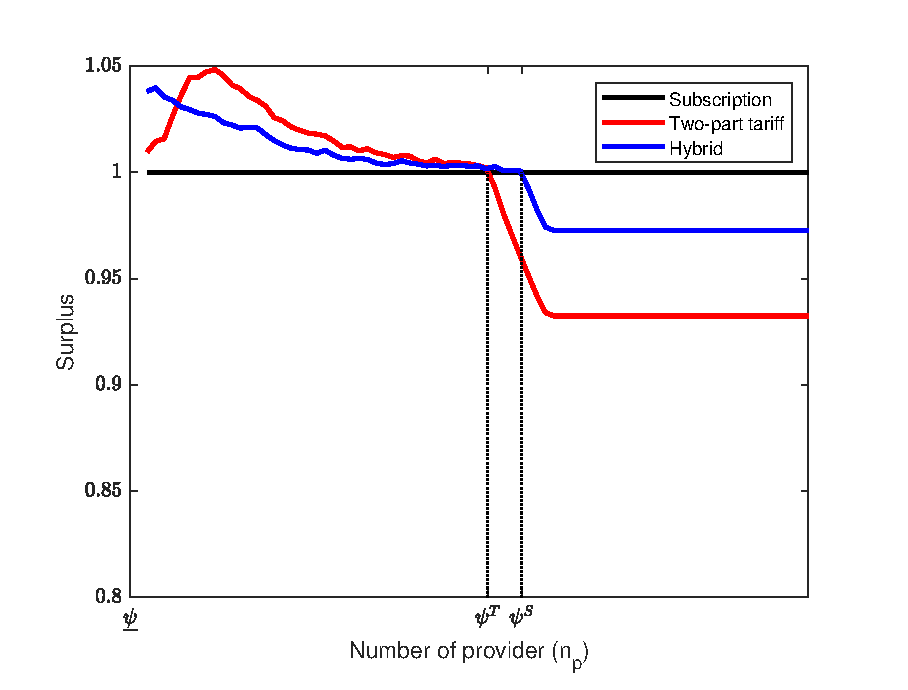
\includegraphics[width=5cm]{figure_3rd_final/prop_c_6_1.eps}}    
    \caption{Numerical Analysis on Heterogeneous Storage Volume (Utility Function I, Scenario ii)}
\end{figure}
%- 아래의 pareto distribution에서 parameter가 달라질 때 효과와 연결\\
%- 용량이 큰 고객의 $b$가 큰 경우에, 이들에게는 i) first-best 인 부분에서 bandwidth에 비용을 지불받는 것의 merit이 줄어들어 subscription과 가까워짐 2) 마찬가지로 market-clearing에서도 bandwidth로부터 얻는 이익이 많이 없어져서 subscription과 가까워짐 -- c로 갈 수록 전체적으로 subscription과 가까워지는 모습(특히, hybrid)\\

\newpage

\textbf{Utility function II.}  When the bandwidth allowance is constant\\
\underline{\textit{Scenario i})} $(b_l, b_h) = (2, 2)$
\begin{figure}[ht!]
\def\figurename{Figure R2 -}
    \centering
    \subfigure[$Low:High = 9:1$]{\includegraphics[width=5cm]{figure_3rd_final/volume_c_1.eps}}
    \subfigure[$Low:High = 5:5$]{\includegraphics[width=5cm]{figure_3rd_final/volume_c_2.eps}}
    \subfigure[$Low:High = 1:9$]{\includegraphics[width=5cm]{figure_3rd_final/volume_c_3.eps}}
    \caption{Numerical Analysis on Heterogeneous Storage Volume (Utility Function II, Scenario i)}
\end{figure}

\underline{\textit{Scenario ii})} $(b_l, b_h) = (2, 5)$
%%%%%%%%%%%%%%%%%%
\begin{figure}[ht!]
\def\figurename{Figure R2 -}
    \centering
    \subfigure[$Low:High = 9:1$]{\includegraphics[width=5cm]{figure_3rd_final/volume_c_4.eps}}
    \subfigure[$Low:High = 5:5$]{\includegraphics[width=5cm]{figure_3rd_final/volume_c_5.eps}}
    \subfigure[$Low:High = 1:9$]{\includegraphics[width=5cm]{figure_3rd_final/volume_c_6.eps}}
    \caption{Numerical Analysis on Heterogeneous Storage Volume (Utility Function II, Scenario ii)}
\end{figure}

\begin{quotation}
{\em
\noindent \textbf{Reviewer 2 (Point A2b): }
b. Compared to the concern on the unit volume of each renter, perhaps the assumption that each provider supplies unit volume of unused capacity is fine. But the implication is that the provider’s income and cost are both proportional to the volume of capacity supplied. If this is most likely the case in the storage sharing industry, the authors need to explain this point to justify this assumption; otherwise, I wonder whether the authors could relax this assumption, i.e., whether the impacts of a specific pricing scheme on providers with different capacity are different.}
\end{quotation}\vspace{-4mm}

This is another great point. As you indicated, we can safely ensure the validity of our findings if each provider's income and cost are both proportional to his storage capacity. Specifically, we set each provider's operating cost to be proportional to $\hat{\omega_b}$ (i.e., the expected bandwidth volume for each provider), and $\hat{\omega_b}$ is proportional to each provider's shared storage capacity. Below, we discuss whether this assumption is consistent with the reality, and potential implications of alternative cost forms.

\textbf{Is the operating cost proportional to $\hat{\omega_b}$?} The operating costs may include various sources, such as Internet bandwidth, electricity costs, and obsolescence of the computing device. Intuitively, bandwidth and electricity costs are proportional to bandwidth usage. Hardware obsolescence is directly related to the computational burden, and it is attributable to both computation amount and running time. Although the exact functional form of this relationship is unknown, its impact tends to be secondary to other direct costs (i.e., bandwidth and electricity) and is partially absorbed by $\xi(t)$. Thus, it is plausible to assume that the operating cost is proportional to $\hat{\omega_b}$.

\textbf{Is $\hat{\omega_b}$ proportional to the provider's capacity?} P2P storage platforms usually encourage providers to share more capacity by mentioning that sharing more capacity will lead to more access from renters and more earnings. Also, it is commonly observed that providers with higher capacity tend to store more files than those with lower capacity on these platforms. Thus, it is plausible to assume that the platform assigns more files and bandwidth services to high-capacity providers than low-capacity ones.

\textbf{How would alternative cost forms affect the results?} Alternative cost functions may affect our main insights as follows. First, we may consider a convex function, such as quadratic and exponential forms, where operating costs are particularly burdensome for high-capacity providers. In this case, as high-capacity providers bear much higher operating costs and join the platform less, the first-best prices will be less achievable. Hence, compensating for offering bandwidth services will have a higher impact on the storage capacity. Consequently, the relative benefits of two-part tariff and hybrid pricing (vs. subscription-based pricing), which mainly come from enhancing the platform's capacity, will be greater in this situation.

Second, we may also consider a concave function of operating costs like a square root function. Since high-capacity providers bear relatively less operating burden than they do in the current setup, the platform will attract more providers under the subscription-based pricing---which does not compensate for offering bandwidth services. Therefore, the profit/surplus gap between the subscription and other pricing schemes will decrease as a result. However, although the magnitudes decline, we expect the differences to remain qualitatively unchanged.

We have summarized this discussion in the revised manuscript as follows:

``Second, one might consider an alternative form of the provider's operating cost. Basically, the current form relies on the assumptions that operating costs are proportional to $\hat{\omega_b}$ (i.e., the expected bandwidth volume for each provider), and that $\hat{\omega_b}$ is proportional to each provider's shared storage capacity. We argue that these assumptions are plausible for the following reasons: 1) many of the major costs, such as Internet bandwidth and electricity costs, are proportional to bandwidth usage, and 2) the platform tends to assign more files and bandwidth services to high-capacity providers than low-capacity ones.

So, how would alternative cost forms affect the results? On the one hand, we may consider a convex function, such as quadratic and exponential forms, where operating costs are particularly burdensome for high-capacity providers. In this case, as high-capacity providers bear much higher operating costs and join the platform less, compensating for offering bandwidth services will have a higher impact on the storage capacity. Consequently, the relative benefits of two-part tariff and hybrid pricing (vs. subscription-based pricing) will be greater in this situation. On the other hand, we may also consider a concave function like a square root function. Since high-capacity providers bear relatively less operating burden than they do in the current setup, the platform will attract more providers under the subscription-based pricing. Hence, the profit/surplus gap between the subscription and other pricing schemes will decrease as a result. However, although the magnitudes decline, we expect the differences to remain qualitatively unchanged.'' (page 25)


%%%%%%%%%%%%%%%%%%%%%%%%%%%%%%%%%%%%%%%%%%%%%%%%%%%%%%%%%%%%%%%

\begin{quotation}
{\em
\noindent \textbf{Reviewer 3 (Point 7): } 2. In a similar vein, it is a little strange that consumer’s usage of the platform is exogenously given instead of responding to the incentives created by the firm’s pricing scheme.
}

이 부분에 대한 답변은 고민해봐야하는데, in-out decision을 위주로 보고 있는 literature들을 여러개 reference해서 이 세팅도 많이 고려되고 있는 형태라는 것을 보여주는 것이 좋지 않을까 싶습니다

\ju{Li and Kumar (2018) (메인으로는 말고) + 몇몇 논문 가져와서 사례가 많이 있다고 언급 + Practical하게 말이 되는 이유...?}

\ju{Newsvendor...고객의 distribution이 있고 거기에 대해 최적 pricing을 결정하는 것...이런 문제들도 의미가 있다}
initial newsvendor model -> p와 independent한 demand distribution 고려\\
참고:
https://en.wikipedia.org/wiki/Newsvendor_model

\begin{quotation}
{\em
\noindent \textbf{Reviewer 2 (Point A4a):  }4. Other model assumptions to justify: a. The assumption about independence of a renter’s utility from the download bandwidth service from her download frequency is questionable. One may argue that the two parameters are positively correlated as the more frequent the renter needs to access the storage, the more valuable the bandwidth service means to her.}
\end{quotation}\vspace{-4mm}

This is another great point. In our analysis, we have postulated that a renter's utility per bandwidth volume is independent of her download frequency. Let us note that among renters adopting the platform, the utility per volume and the download frequency are already positively associated with each other as a result of self-selection. In this regard, if the two parameters are positively correlated among all potential renters, we will obtain a more dramatic relationship among platform-adopting renters. Therefore, we expect that the implications of pricing schemes will be qualitatively consistent.

We have validated this conjecture by examining a scenario where potential renters with the higher utility per download volume tend to have more frequent download requests. We have manipulated the shape parameter $b$ of the Pareto distribution---which determines the extent to which the bandwidth frequency is concentrated or dispersed---differently by the utility per bandwidth volume. Specifically, we have divided potential renters into two groups: 1) renters whose unit utility is uniformly distributed in $[0, 0.5]$ and whose frequency follows the Pareto distribution having a lighter tail (with $b_l=5$), and 2) those whose unit utility is uniformly distributed in $[0.5, 1]$ and whose frequency follows the Pareto distribution having a heavier tail (with $b_h=2$), where $b_l > b_h$. For this scenario, we have conducted a numerical analysis and obtained qualitatively similar results (see \textbf{Figure R2-5}).

\begin{figure}[ht!]
\def\figurename{Figure R2 -}
\centering
\includegraphics[width=8cm]{figure_3rd_final/half_1.eps} 
\caption{Numerical Analysis on Positive Association Between Utility per Download and Download Frequency. The red (blue) line indicates the relative total surplus of the two-part tariff (the hybrid pricing) compared with the subscription-based pricing, which is represented as the horizontal black line.}
\end{figure}

The revised manuscript provides a summary of this discussion as below :

``Also, our model postulates that the distributions of the utility per bandwidth volume and the download frequency are independent. Although this leads to a positive association between these variables as a result of self-selection, it is also possible that they are positively associated with each other before the renter's decision. We examine whether the implications of pricing schemes are qualitatively consistent after relaxing this assumption by conducting a numerical study. We observe that our main findings remain qualitatively consistent.'' (page 26)

\begin{quotation}
{\em
\noindent \textbf{Reviewer 2 (Point A4b):  }b. The assumption that the renters’ bandwidth usage level follows a Pareto distribution needs better justification. Are there other studies (or empirical evidence) than Li and Kumar (2018) that also adopt this assumption? Can the same results be derived based on other distributions (e.g., Poisson)?}
\end{quotation}\vspace{-4mm}

We apologize that we did not sufficiently justify our using a Pareto distribution. In adherence to your comments, we have added prior studies that adopted this assumption and examined whether our results are restricted to the heavy tail distribution in this revision.

In our description of the related literature, we have supplemented prior studies that utilized the Pareto distribution following the empirical findings of Loboz (2012). Moreover, we have provided additional examples showing that digital consumption is likely to have heavy-tailed distributions. The following presents our revised paragraph:

``This model concerns renters with a continuum of bandwidth usage level (or frequency of download requests) of stored files denoted by $\lambda$. It has been empirically observed in the literature that the usage of cloud-resource is distributed with relatively heavy tails compared with exponential, log-normal, and normal distributions (Loboz, 2012), similarly to other digital resources like smartphone and YouTube usage (Falaki et al., 2010; Gill et al., 2008). Thus, we assume that a renter’s bandwidth usage $\lambda$ follows the Pareto distribution in keeping with the extant literature (Bandi et al., 2015; Li and Kumar, 2018; Ramírez-Velarde et al., 2017).'' (page 9)

%시나리오 1. pareto 밖에 안될 경우 -> 우리가 renter의 frequency 분포가 달라지는 경우들을 여러가지로 고려해보기 위하여, 기존의 shape parameter와 다른 b 값을 넣어서 테스트를 해보았다. (이 경우에는 b값에 따라 달라지는 pareto distribution을 그래프 혹은 표로 + 정보로 넣는것도 방법일듯?) 그럼에도 불구하고 똑같았다. 

%시나리오 2. 다 될 경우 -> 다 해봤다. 똑같았다.

Although the heavy-tail assumption has been empirically confirmed, the exact shape might vary across contexts and affect the results differently. To assess whether our results are restricted to the current parameter, we have conducted a numerical analysis for different shapes of distributional tails. We have varied the Pareto's shape parameters and tested whether our findings hold. The results in \textbf{Figure R2-6}) suggest that, in line with the insights from our closed-form results, the total surplus of the two-part tariff and the hybrid pricing can be higher (lower) than the subscription-based pricing when the number of potential providers is small (large).

% \begin{figure}[ht!]
% \centering
% \includegraphics[width=8cm]{figure_3rd_final/f_main_modify.eps} 
% \caption{main}
% \end{figure}
%%%%%%%%%%%%%%%%%%%%%%%
\begin{figure}[ht!]
\def\figurename{Figure R2 -}
    \centering
    \subfigure[$b = 3$]{\includegraphics[width=5cm]{figure_3rd_final/main_3.eps}}
    \subfigure[$b=4$]{\includegraphics[width=5cm]{figure_3rd_final/main_4.eps}}
    \subfigure[$b=5$]{\includegraphics[width=5cm]{figure_3rd_final/main_5.eps}}    
    \caption{Numerical Analysis on Different Parameters of the Pareto Distribution. The red (blue) line indicates the relative total surplus of the two-part tariff (the hybrid pricing) compared with the subscription-based pricing, which is represented as the horizontal black line.}
\end{figure}
%%%%%%%%%%%%%%%%%%%%%%%
% 그래프 설명:\\
% $b$가 커짐에 따라서 two-part tariff, hybrid가 subscription에 가까워짐. \\
% $b$가 커진다는 것은 높은 사용량을 가지는 renter들의 비중이 적다는 뜻. \\
% 따라서 이 경우에 발생하는 현상은 두 가지 dimension으로 설명 가능.\\
% i) bandwidth에 대하여 비용을 부과하는 방식에는 당연히 사용량이 많은 renter들이 더 큰 영향을 받음. 따라서, 사용량이 많은 고객이 적어질 수록, bandwidth price 부과로 인하여 surplus가 감소하는 고객들도 줄어듬. 이로 인해 first-best 범위 내에서도 surplus 발생하는 차이가 줄어들게 됌.\\

% bandwidth에 비용을 부과하는 hybrid, two-part tariff를 통하여 provider에게 충분한 보상이 제공되어, provider을 확보하는데 도움이 되는 logic 자체는 bandwidth를 많이 사용하는 renter들이 많아서 pricing scheme을 변경함으로써 provider에게 더 많은 보상을 제공할 수 있을 때 극대화되는 효과. 따라서, $b$가 커져서 bandwidth를 많이 사용하는 고객들이 줄어드는 상황에서는 hybrid 및 two-part tariff가

We have discussed this point in the new version as follows:

``First, we find that our findings remain consistent when we relax the assumption of bandwidth usage distribution. 
Specifically, we assume that bandwidth usage follows the Pareto distribution with $b=2$ to account for the heavy-tail distribution and analytical tractability. To assess whether this assumption is entirely responsible for our findings, we conduct a numerical analysis of different shapes of distributional tails. For ease of comparison, we have varied the Pareto’s shape parameters and tested whether our findings hold. The results show that the implications of pricing schemes do not change under different parametric conditions.'' (pages 25-26)




\end{quotation}\vspace{-4mm}



\end{document} 
